\documentclass[12 pt]{extarticle}

	\usepackage[frenchb]{babel}
	\usepackage[utf8]{inputenc}  
	\usepackage[T1]{fontenc}
	\usepackage{amssymb}
	\usepackage[mathscr]{euscript}
	\usepackage{stmaryrd}
	\usepackage{amsmath}
	\usepackage{tikz}
	\usepackage[all,cmtip]{xy}
	\usepackage{amsthm}
	\usepackage{varioref}
	\usepackage{geometry}
	\geometry{a4paper}
	\usepackage{lmodern}
	\usepackage{hyperref}
	\usepackage{array}
	 \usepackage{fancyhdr}
%\renewcommand{\theenumi}{\alph{enumi})}
	\pagestyle{fancy}
	\theoremstyle{plain}
	\fancyfoot[C]{} 
	\fancyhead[L]{Contrôle}
	\fancyhead[R]{13 mai 2024}\geometry{
 a4paper,
 total={180mm,277mm},
 left=20mm,
 top=20mm,
 }
	
	
	\title{Applications de la similitude}
	\date{}
	\begin{document}

 \subsection*{Exercice 1 }
 Dans le triangle ABC, on a $\widehat{BAC}=32^o$ et $\widehat{ABC}= 43^o$. Dans le triangle EFG, on a $\widehat{FEG} = 105^o$ et $\widehat{EFG}= 32^o$. Déterminer si ABC et EFG sont semblables.
 
 
 \subsection*{Exercice 2 }

ABC est un triangle tel que $AB = 8$ cm, $BC = 5$ cm et $AC = 6 cm$. $EFG$ est un triangle avec $EF = 18$ cm, $FG = 15$ cm, et $EG = 24$ cm. \begin{enumerate}
\item 
 Montrer que les triangles sont semblables.
 \item On donne l'aire du triangle $ABC$ est d'environ $15$ centimètres carré. Donner l'aire du triangle $EFG$. 
\end{enumerate}
 \subsection*{Exercice 3}
 
 Soit $ABC$ un triangle rectangle en $A$, avec $BC = 13$ cm et $AC = 12$ cm. 
 \begin{enumerate}
 \item Calculer la longueur $AB$. 
 \item On place sur $[AB]$ le point $D$ tel que $AD= 2$ cm. On place sur $[AC]$ le point $E$ tel que $AE= 4,8$ cm. Faire une figure. 
 \item Montrer que les triangles $ABC$ et $ADE$ sont semblables, et calculer la longueur $DE$.
\end{enumerate}  

 \subsection*{Exercice 4}
 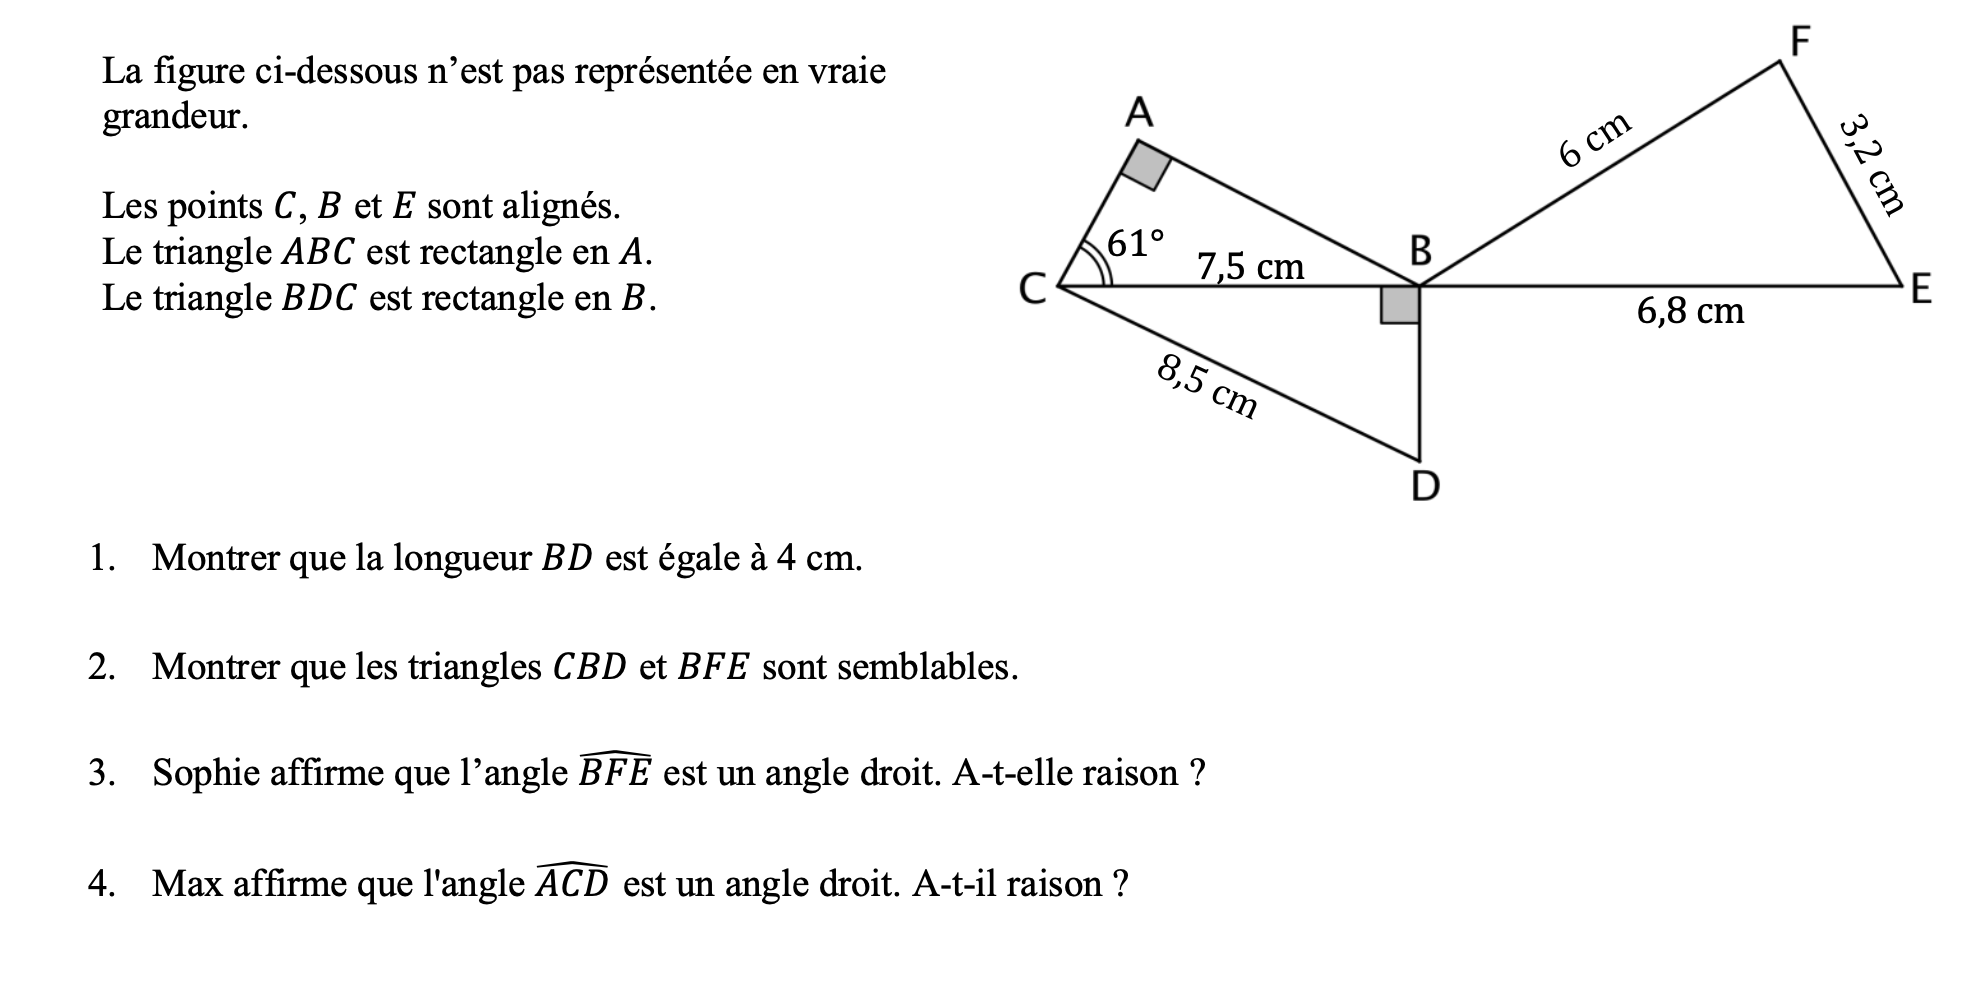
\includegraphics[width = 18 cm]{Exo3}


 
 
 	\end{document}
